\begin{figure}[hbtp]
\centering
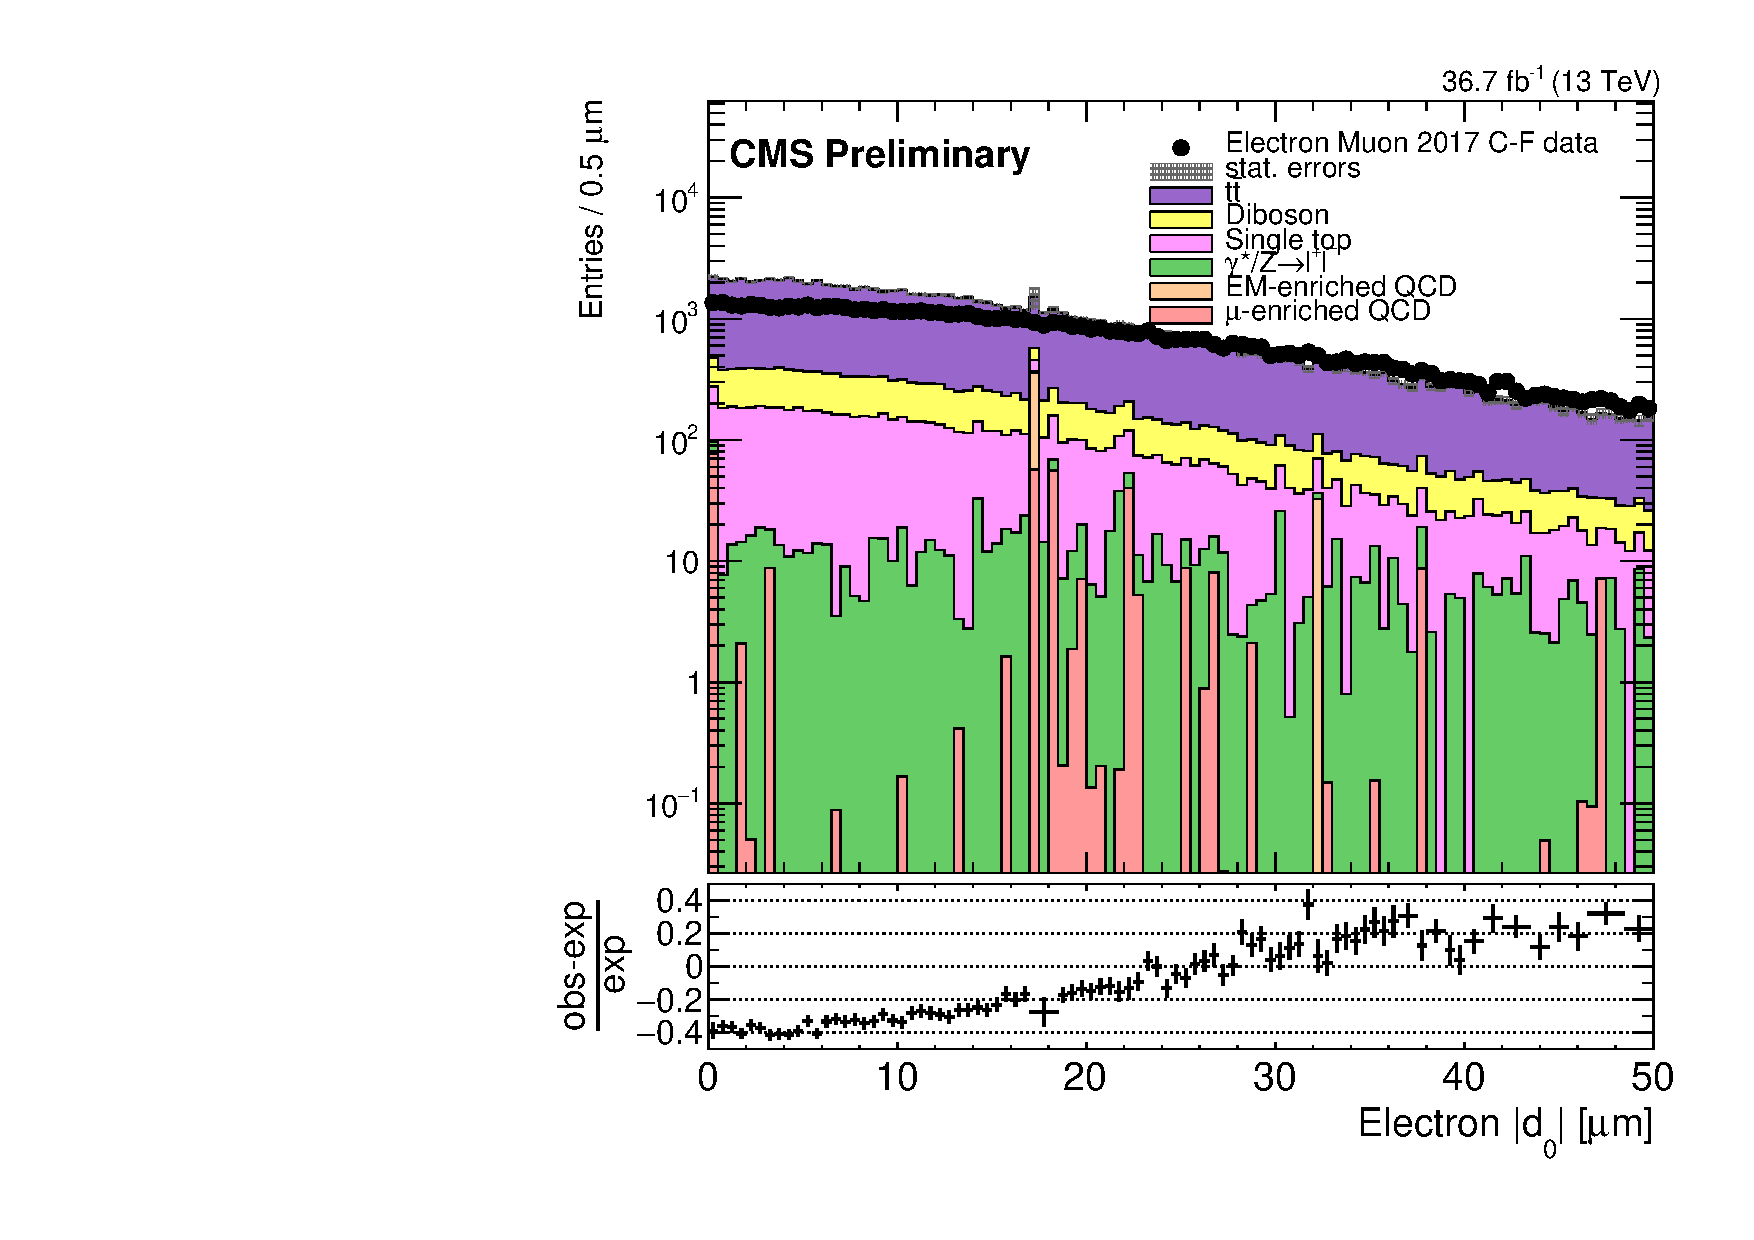
\includegraphics[scale=0.3]{figures/corrections/d0_smearing/emu_2017/electronAbsD0_50um_uncorrected.pdf} 
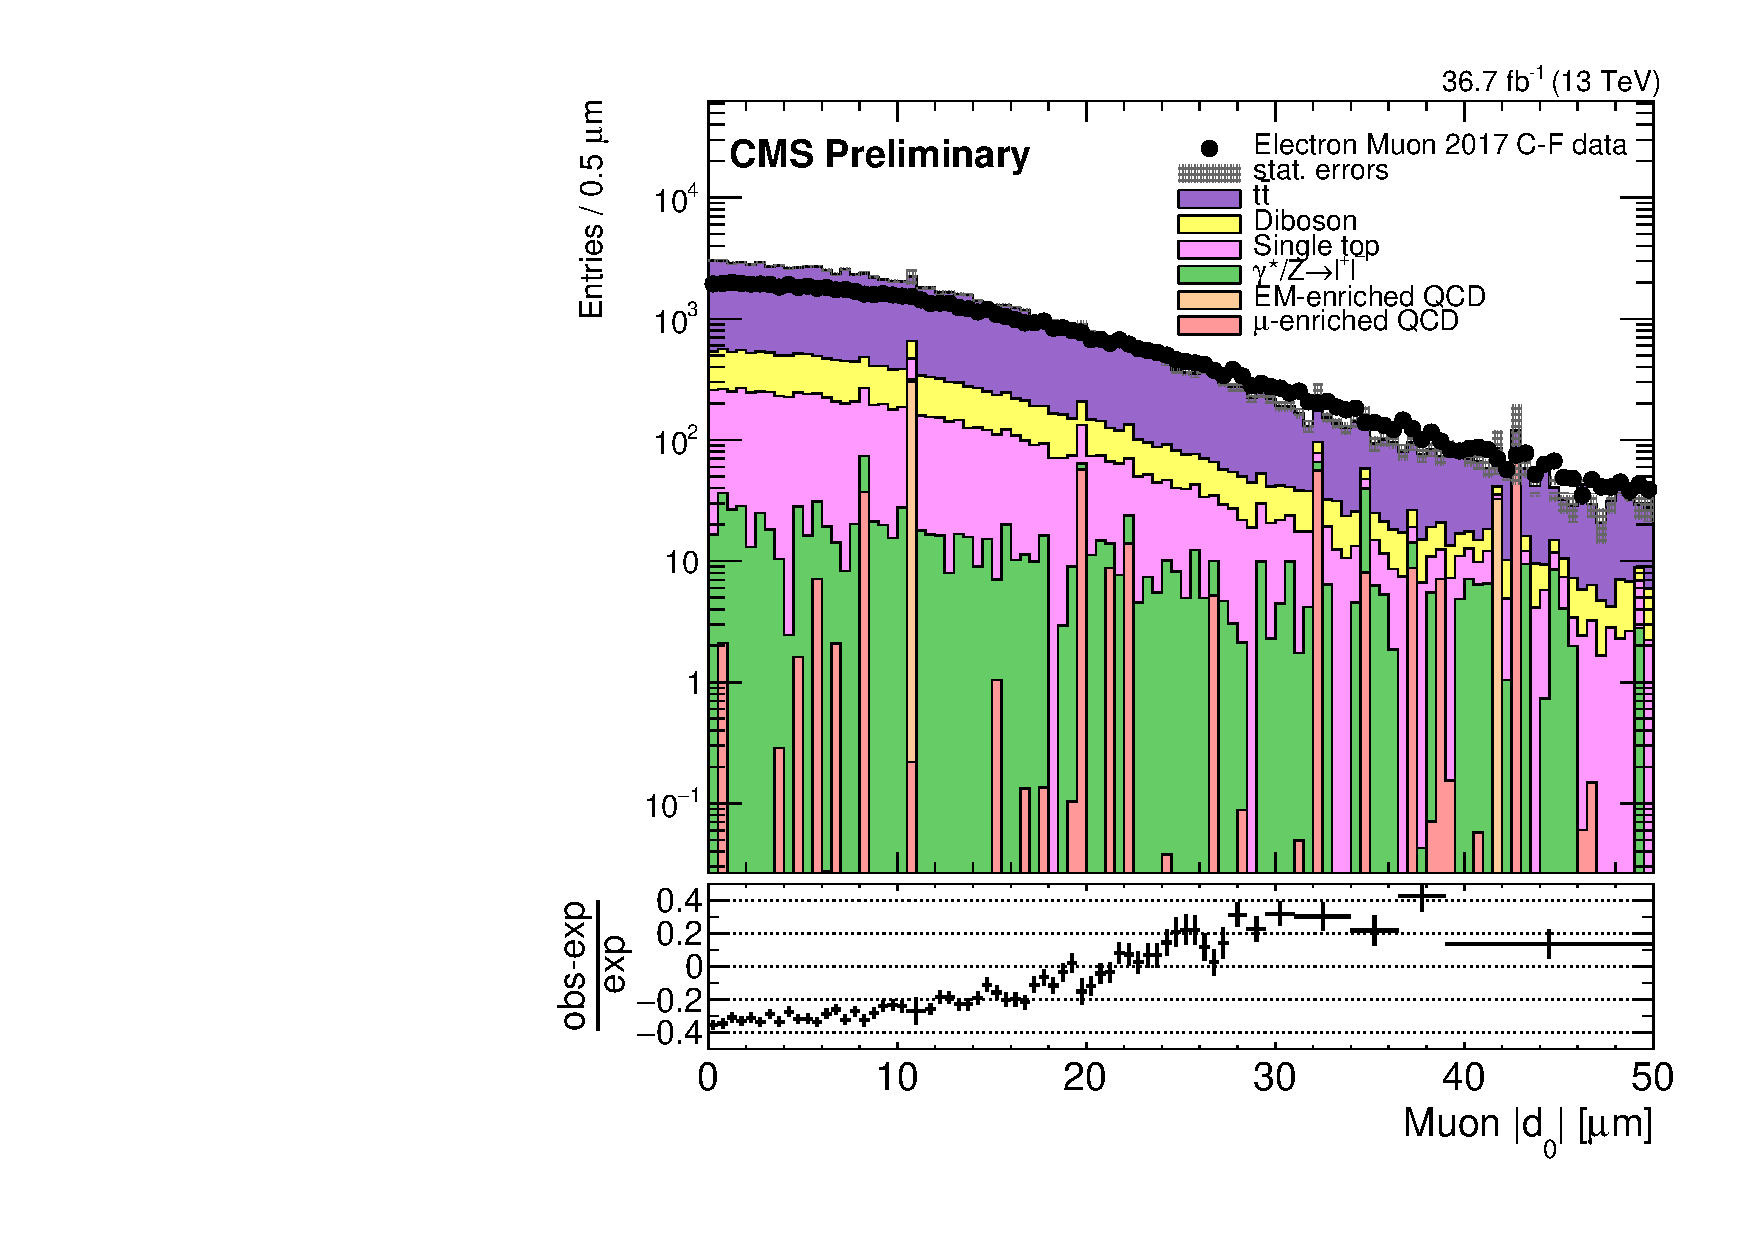
\includegraphics[scale=0.3]{figures/corrections/d0_smearing/emu_2017/muonAbsD0_50um_uncorrected.pdf}
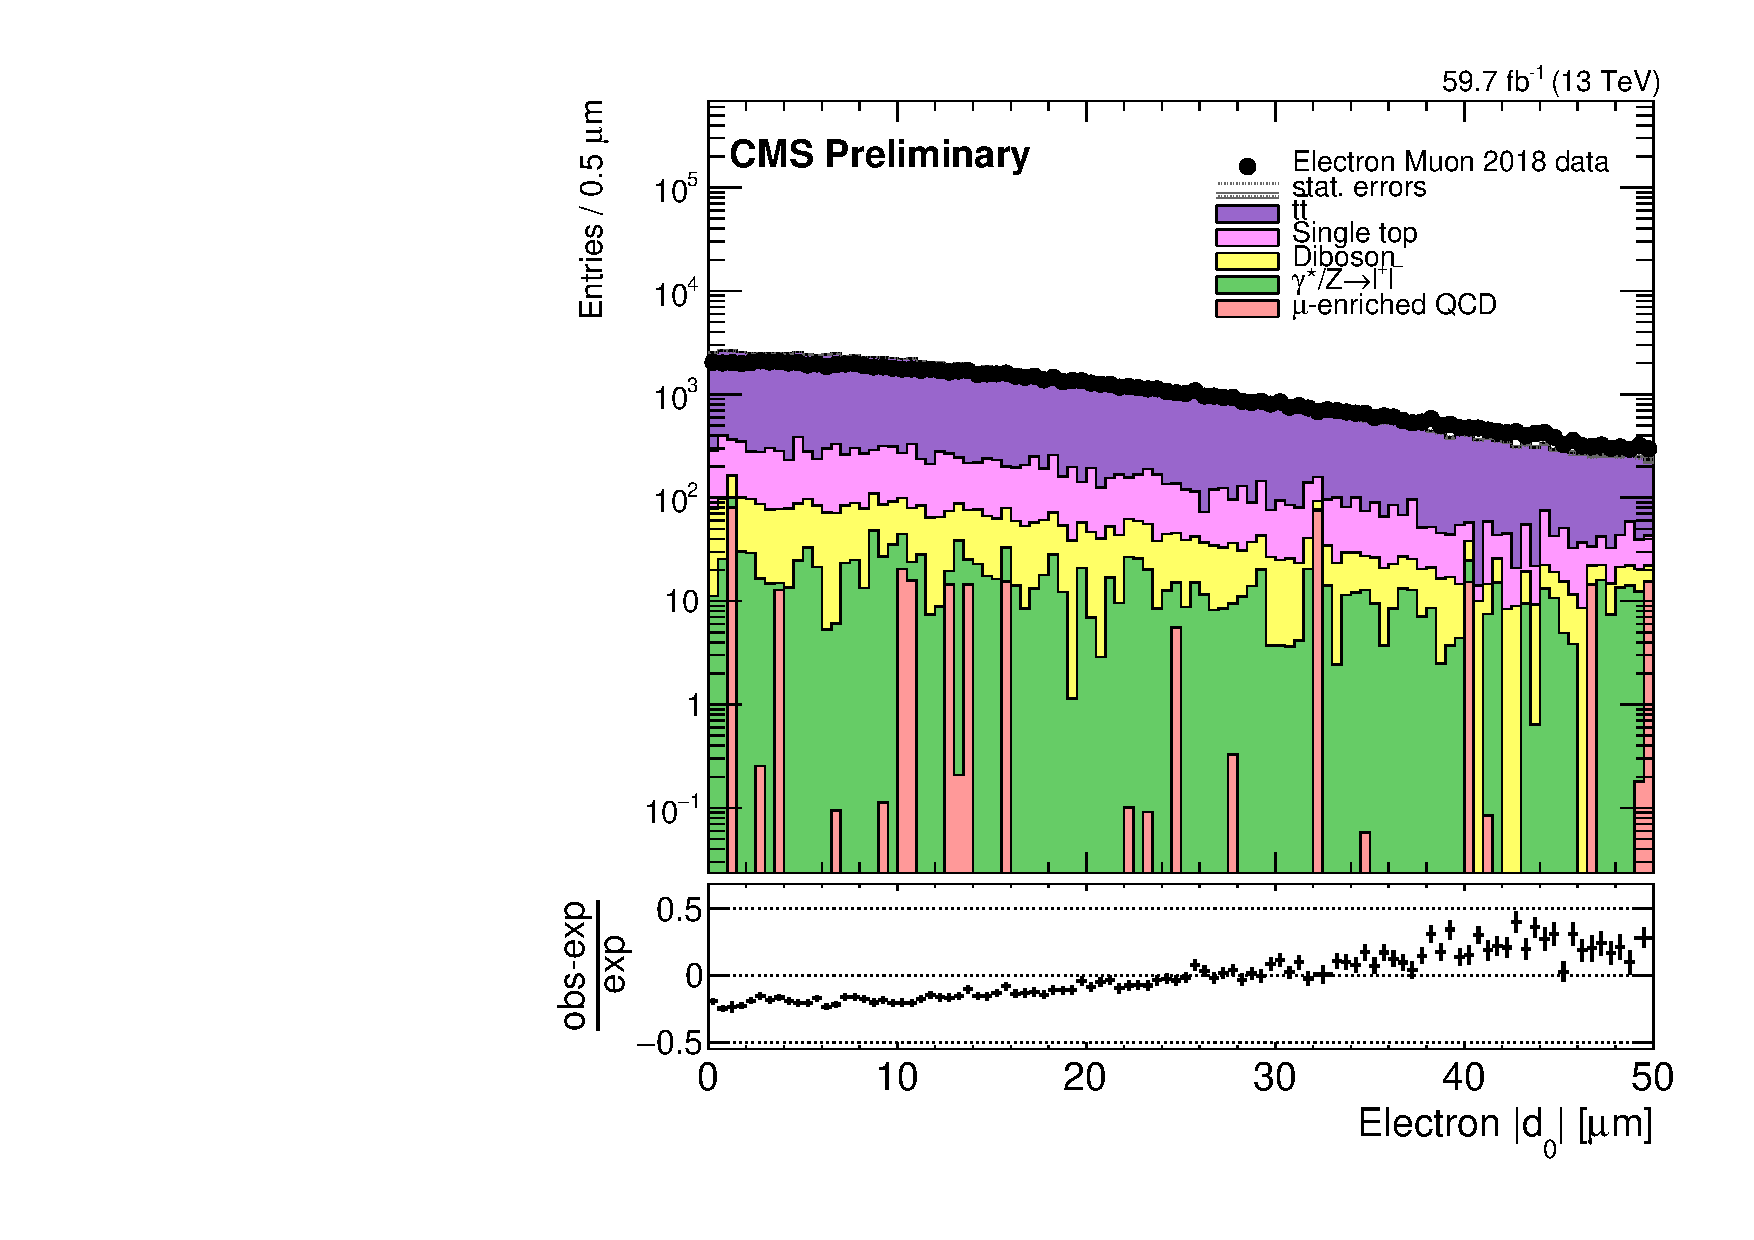
\includegraphics[scale=0.3]{figures/corrections/d0_smearing/emu_2018/electronAbsD0_50um_uncorrected.pdf} 
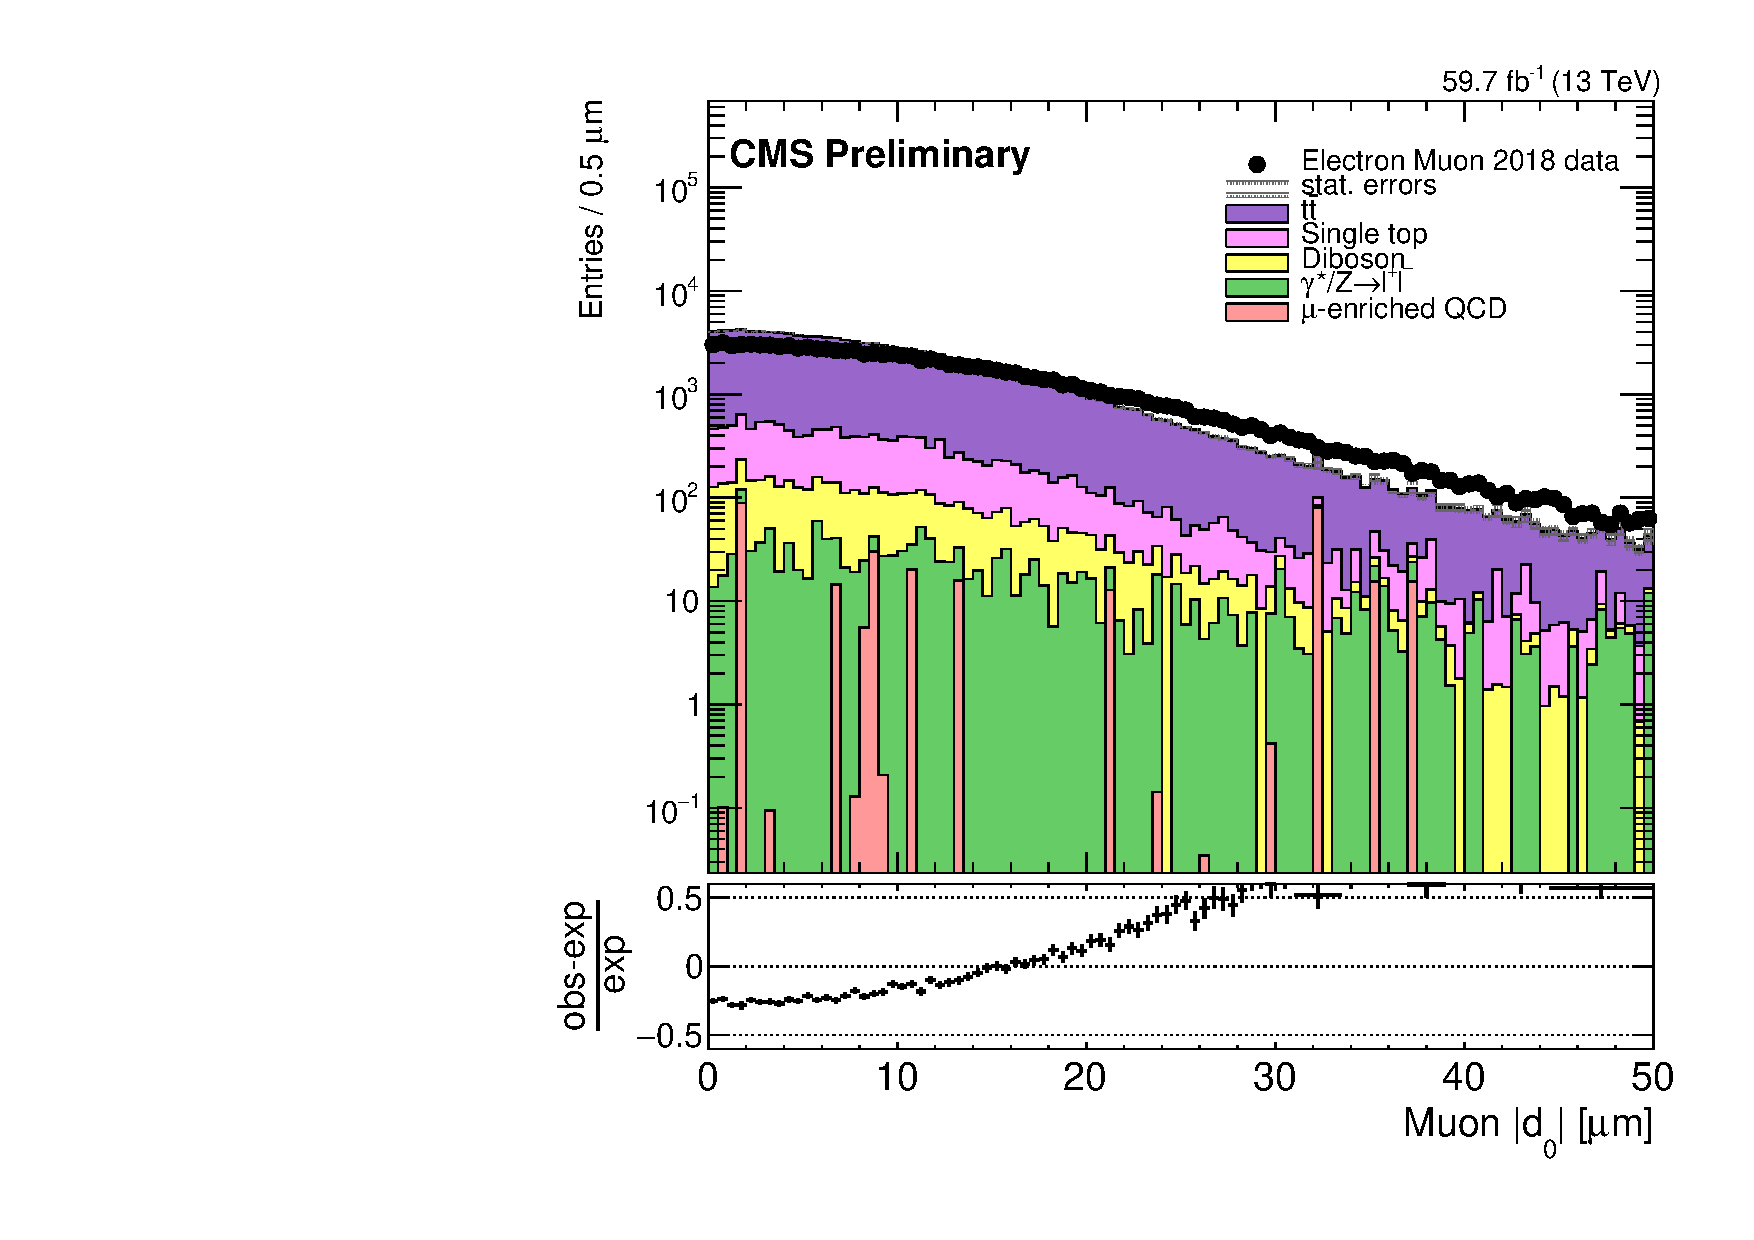
\includegraphics[scale=0.3]{figures/corrections/d0_smearing/emu_2018/muonAbsD0_50um_uncorrected.pdf}
\caption{The uncorrected lepton \ad distributions in the $\Pe\Pgm$ prompt control region, for electrons (left) and muons (right), for 2017 data and simulation (upper), and 2018 data and simulation (lower). The rightmost bin in each plot
contains the overflow entries.}
\label{uncorrected_d0}
\end{figure}

\begin{figure}[hbtp]
\centering
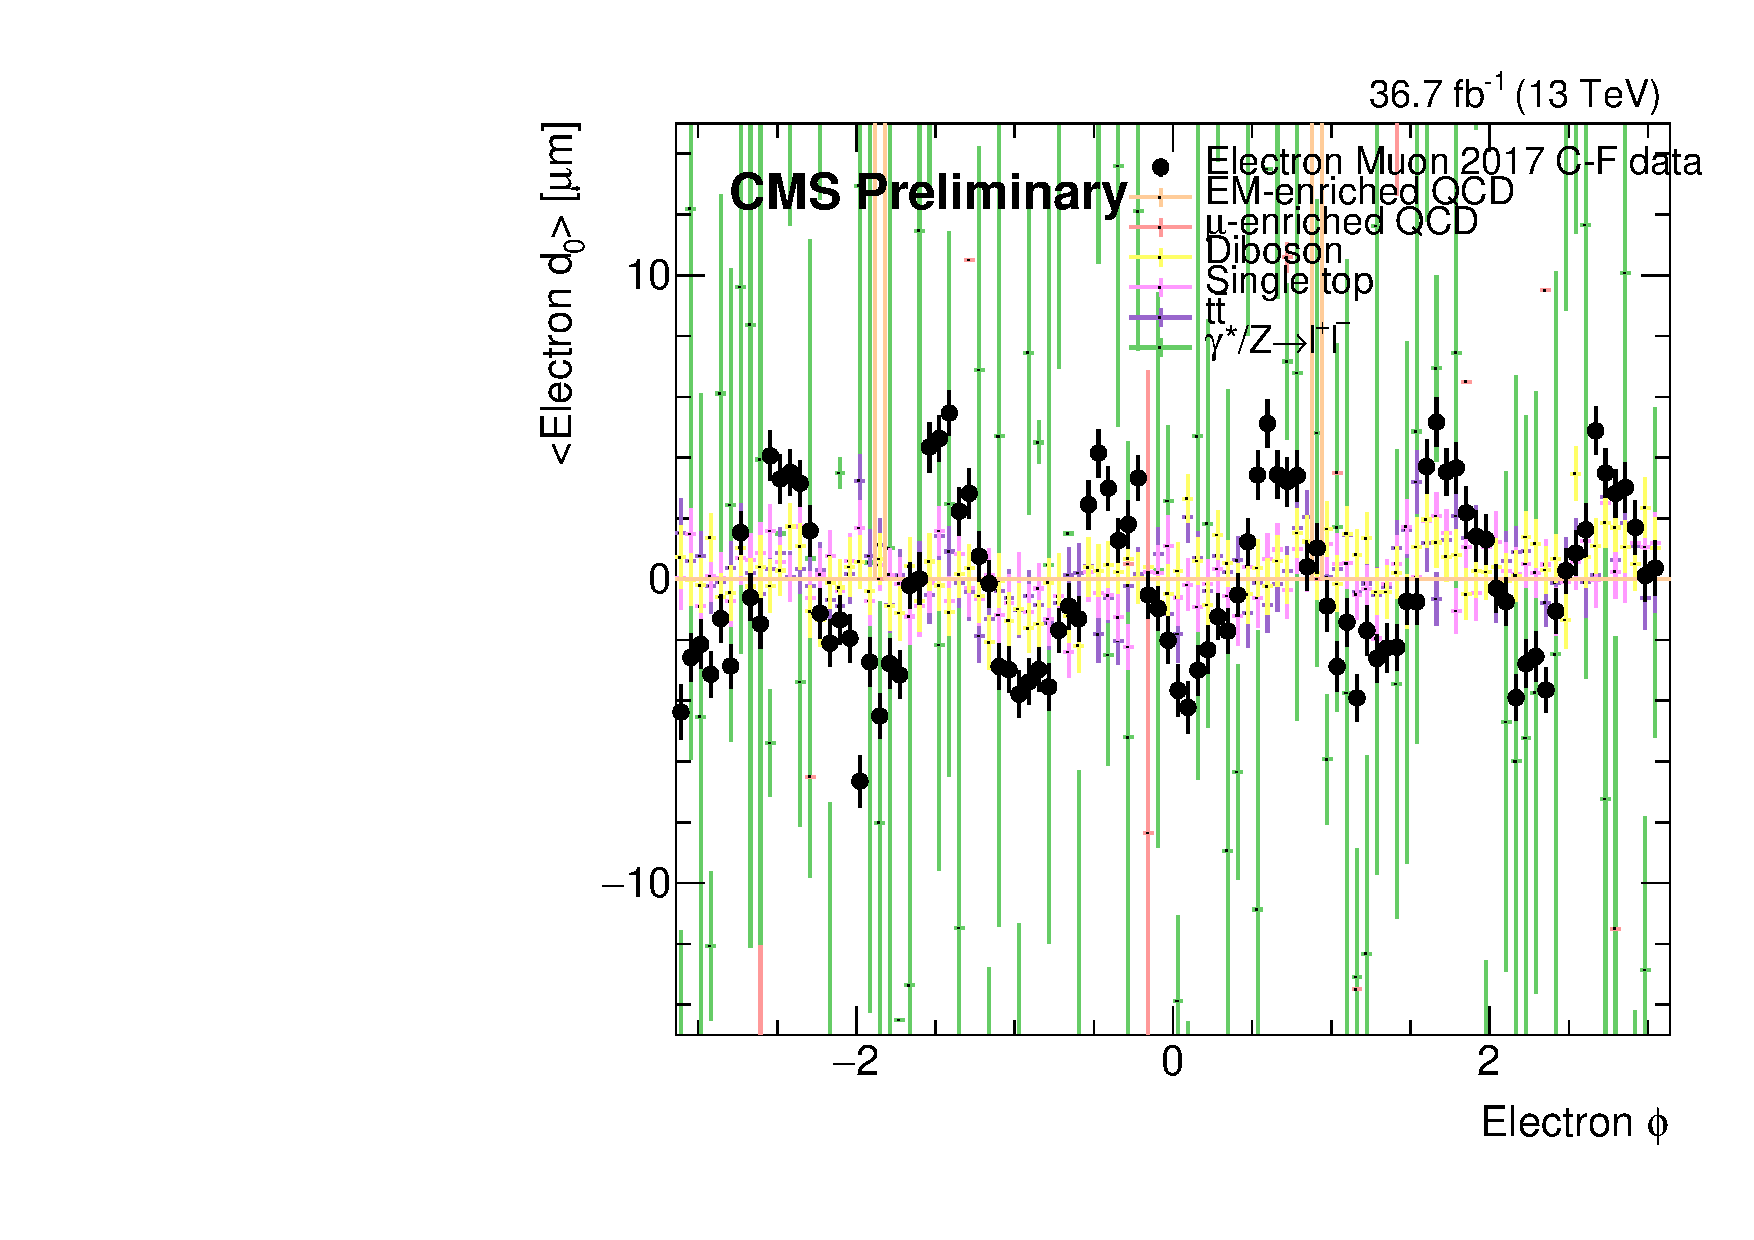
\includegraphics[scale=0.3]{figures/corrections/d0_smearing/emu_2017/electronD0_50um_vs_electronPhi_pfx.pdf}
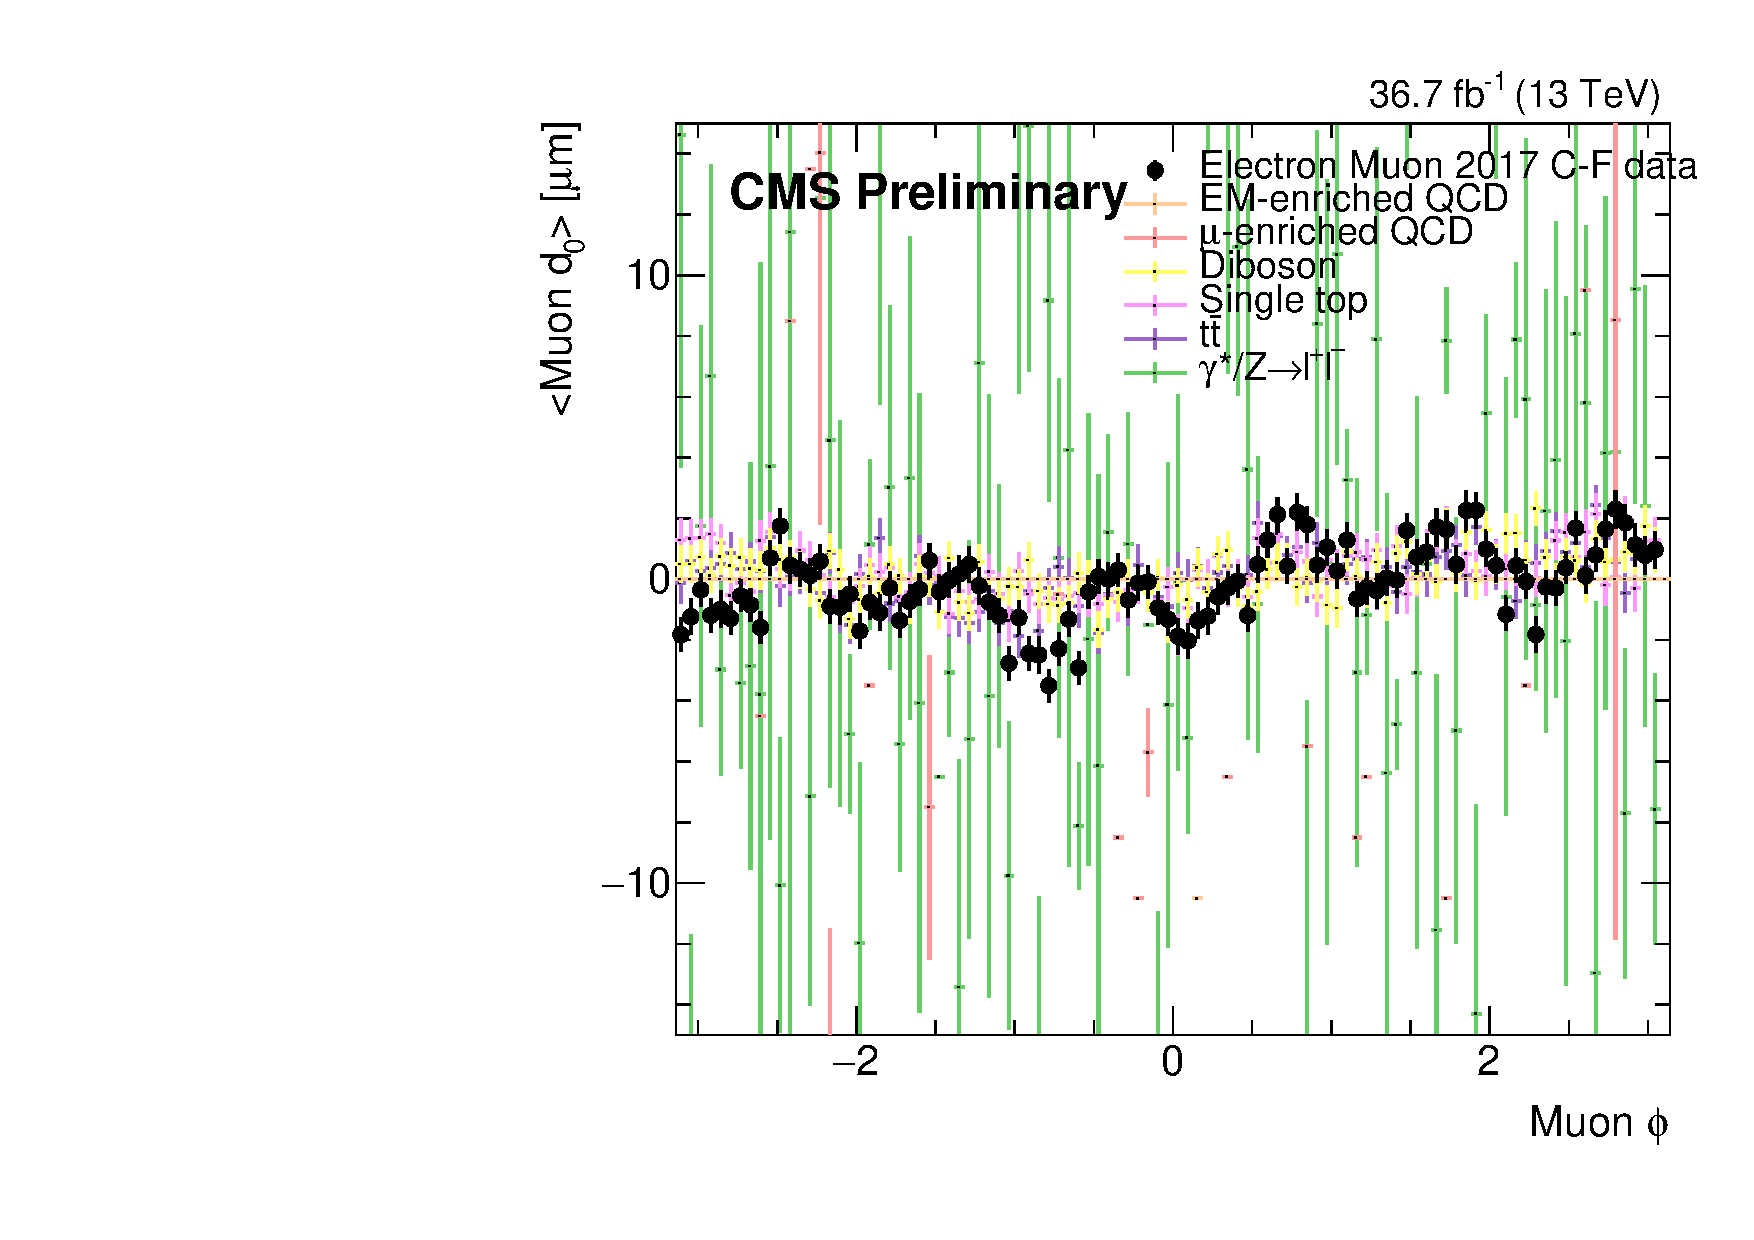
\includegraphics[scale=0.3]{figures/corrections/d0_smearing/emu_2017/muonD0_50um_vs_muonPhi_pfx.pdf}
\caption{The average lepton \ad as a function of $\phi$ in the $\Pe\Pgm$ prompt control region, for electrons (left) and muons (right), for 2017 data and simulation.}
\label{uncorrected_avg_d0_vs_phi}
\end{figure}

\begin{figure}[hbtp]
\centering
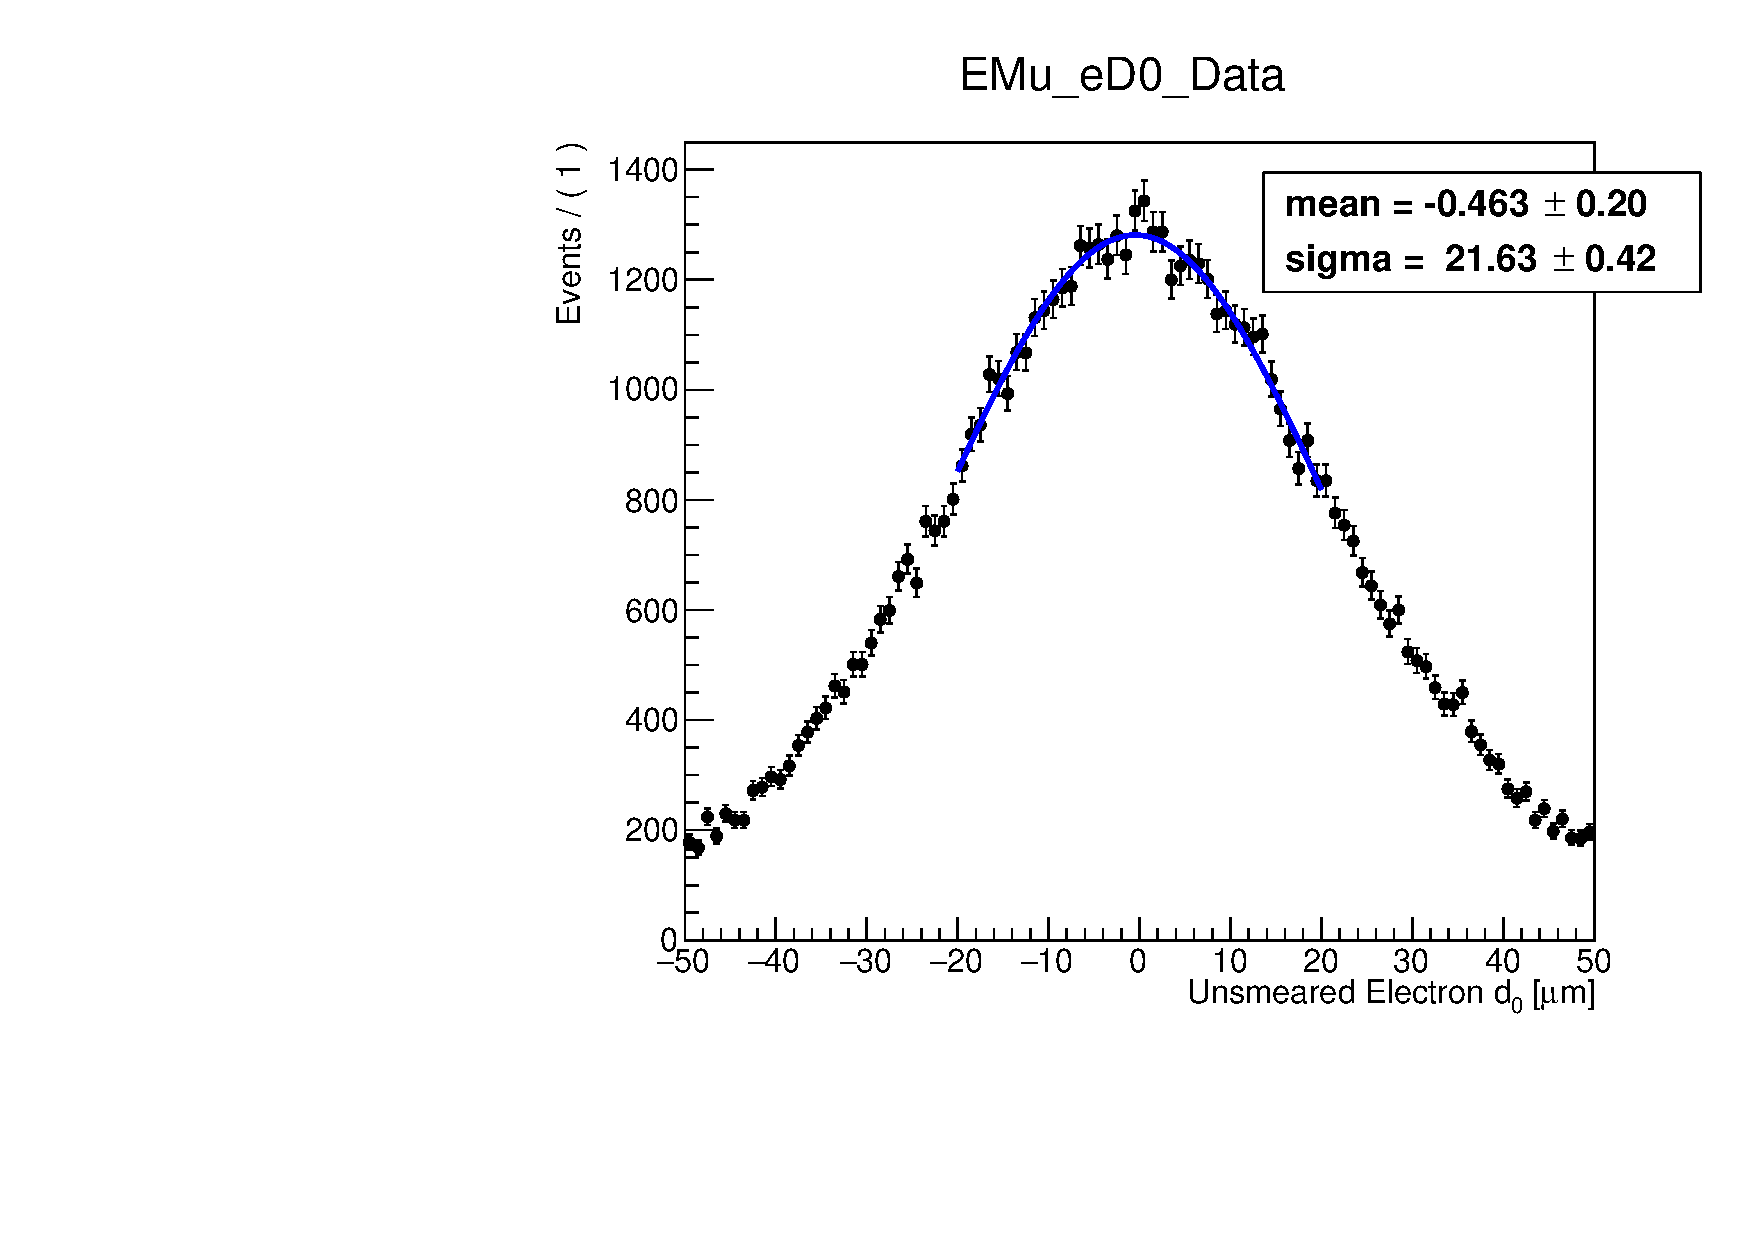
\includegraphics[scale=0.3]{figures/corrections/d0_smearing/emu_2017/gaussian_fit_EMu_eD0_Data.pdf}
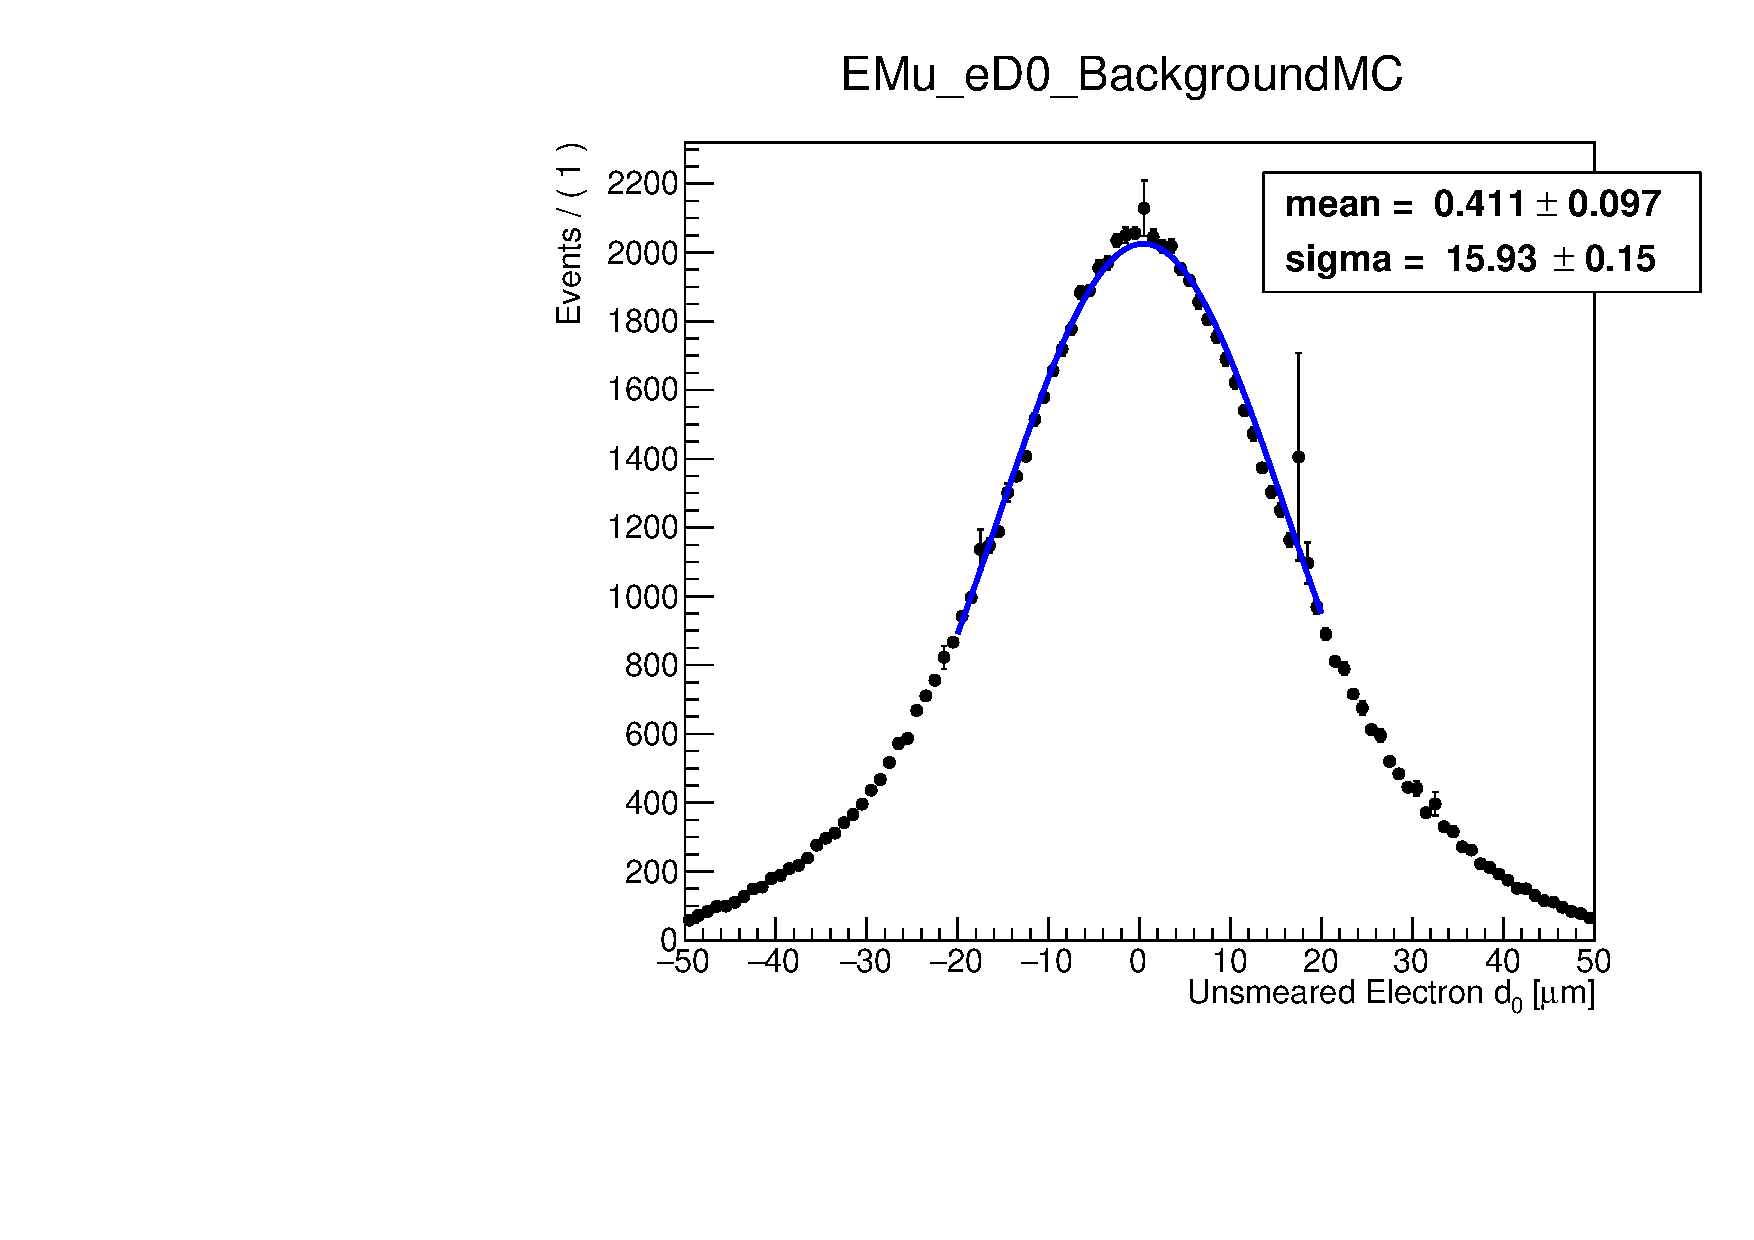
\includegraphics[scale=0.3]{figures/corrections/d0_smearing/emu_2017/gaussian_fit_EMu_eD0_BackgroundMC.pdf}
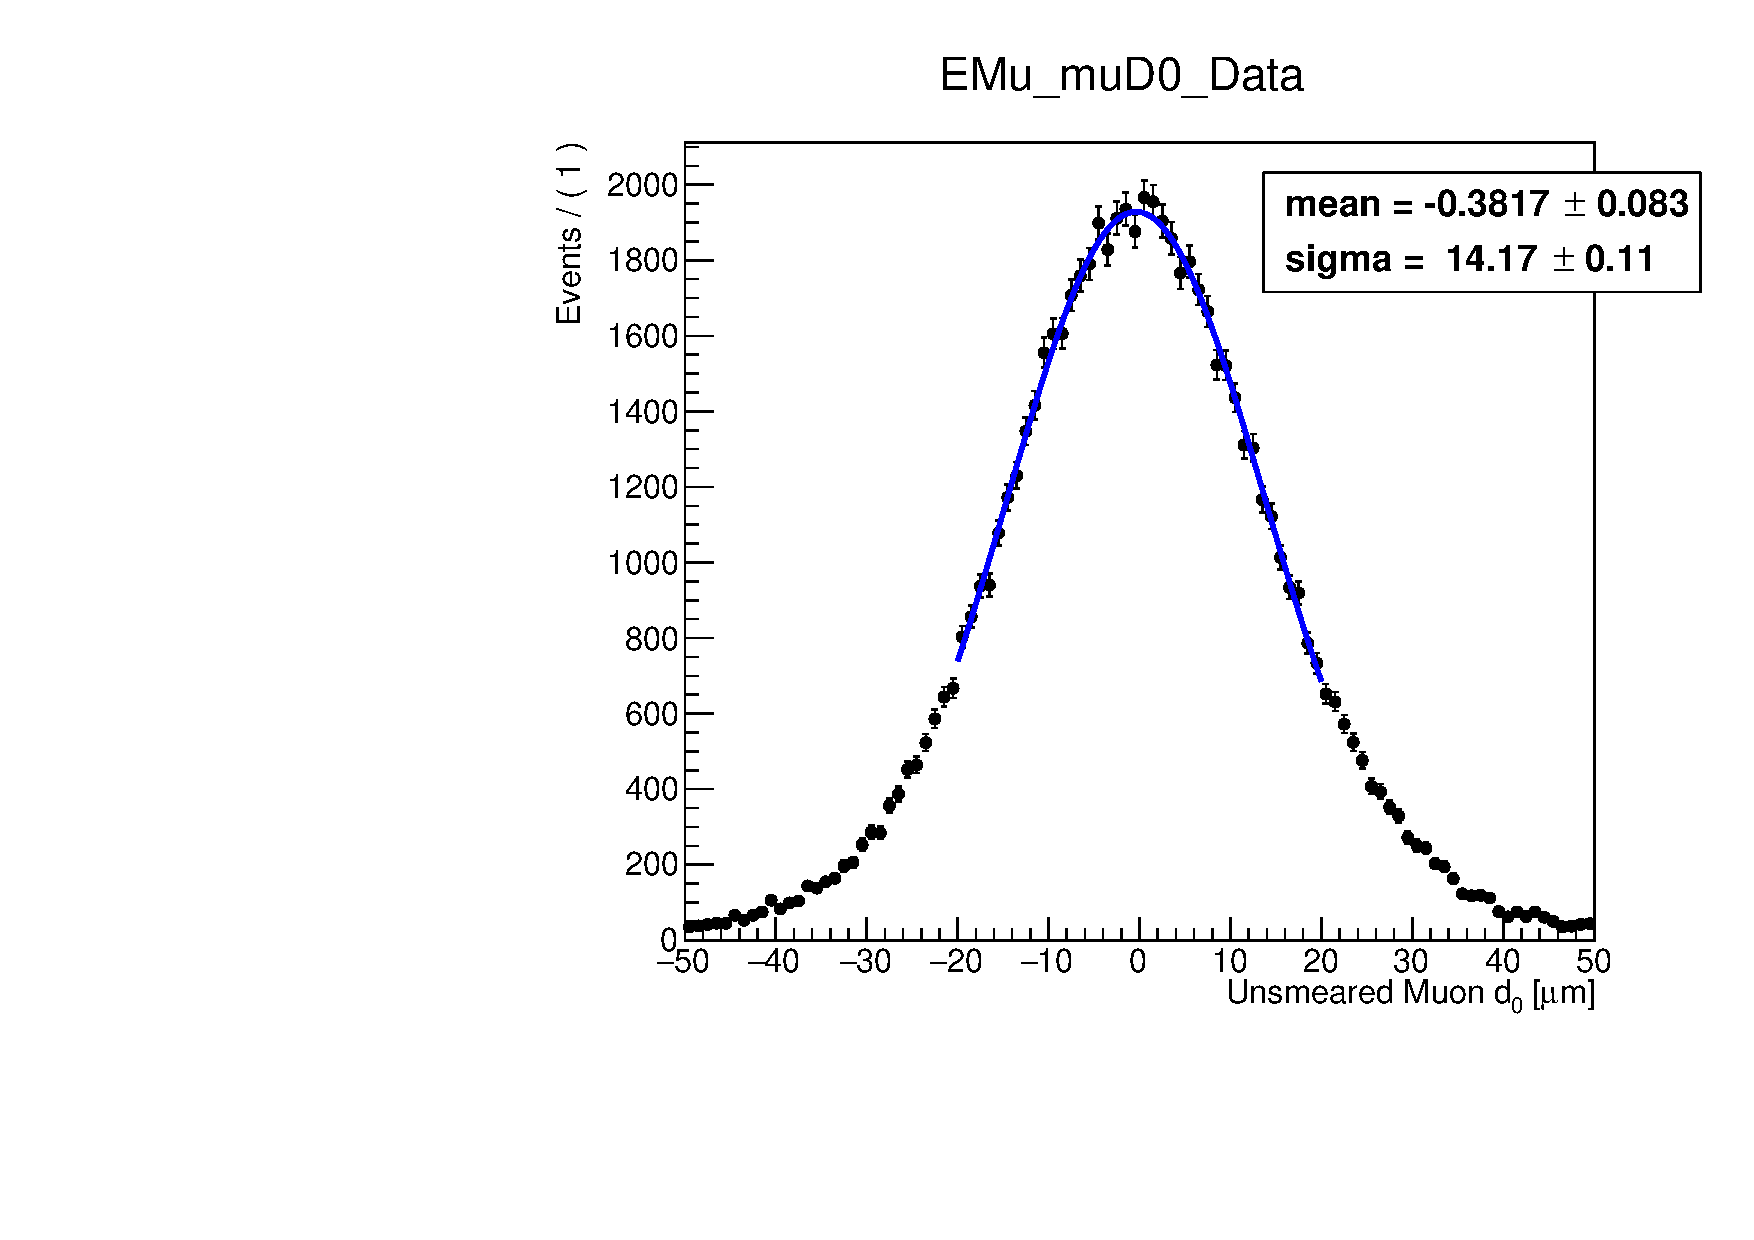
\includegraphics[scale=0.3]{figures/corrections/d0_smearing/emu_2017/gaussian_fit_EMu_muD0_Data.pdf} 
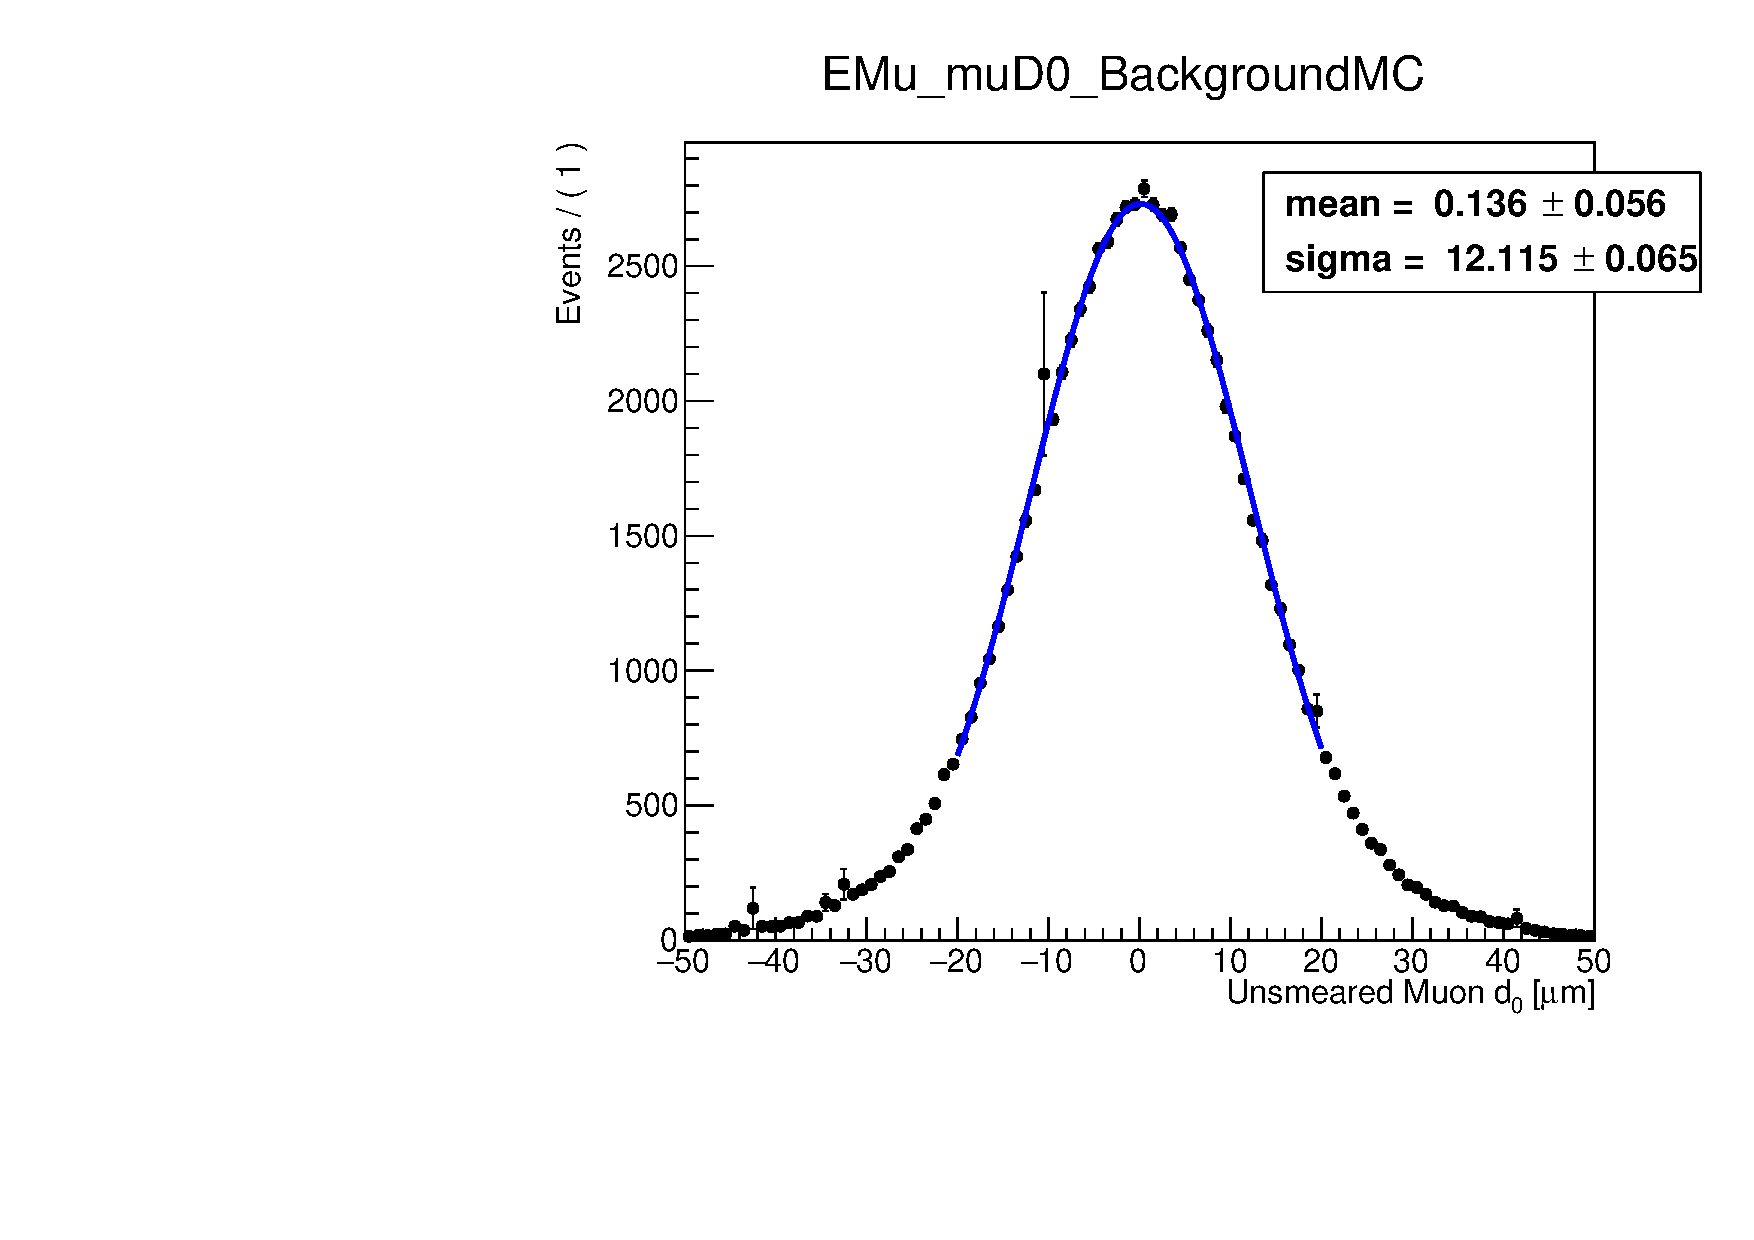
\includegraphics[scale=0.3]{figures/corrections/d0_smearing/emu_2017/gaussian_fit_EMu_muD0_BackgroundMC.pdf}
\caption{The lepton $d_0$ distributions with Gaussian fits in data (left) and background simulation (right) for electrons (upper) and muons (lower) in the 2017 $\Pe\Pgm$ prompt control region. The widths of the Gaussian fits are used to determine the width of the Gaussian distribution used to smear the $d_0$.}
\label{gaussian_fits_2017}
\end{figure}

\begin{figure}[hbtp]
\centering
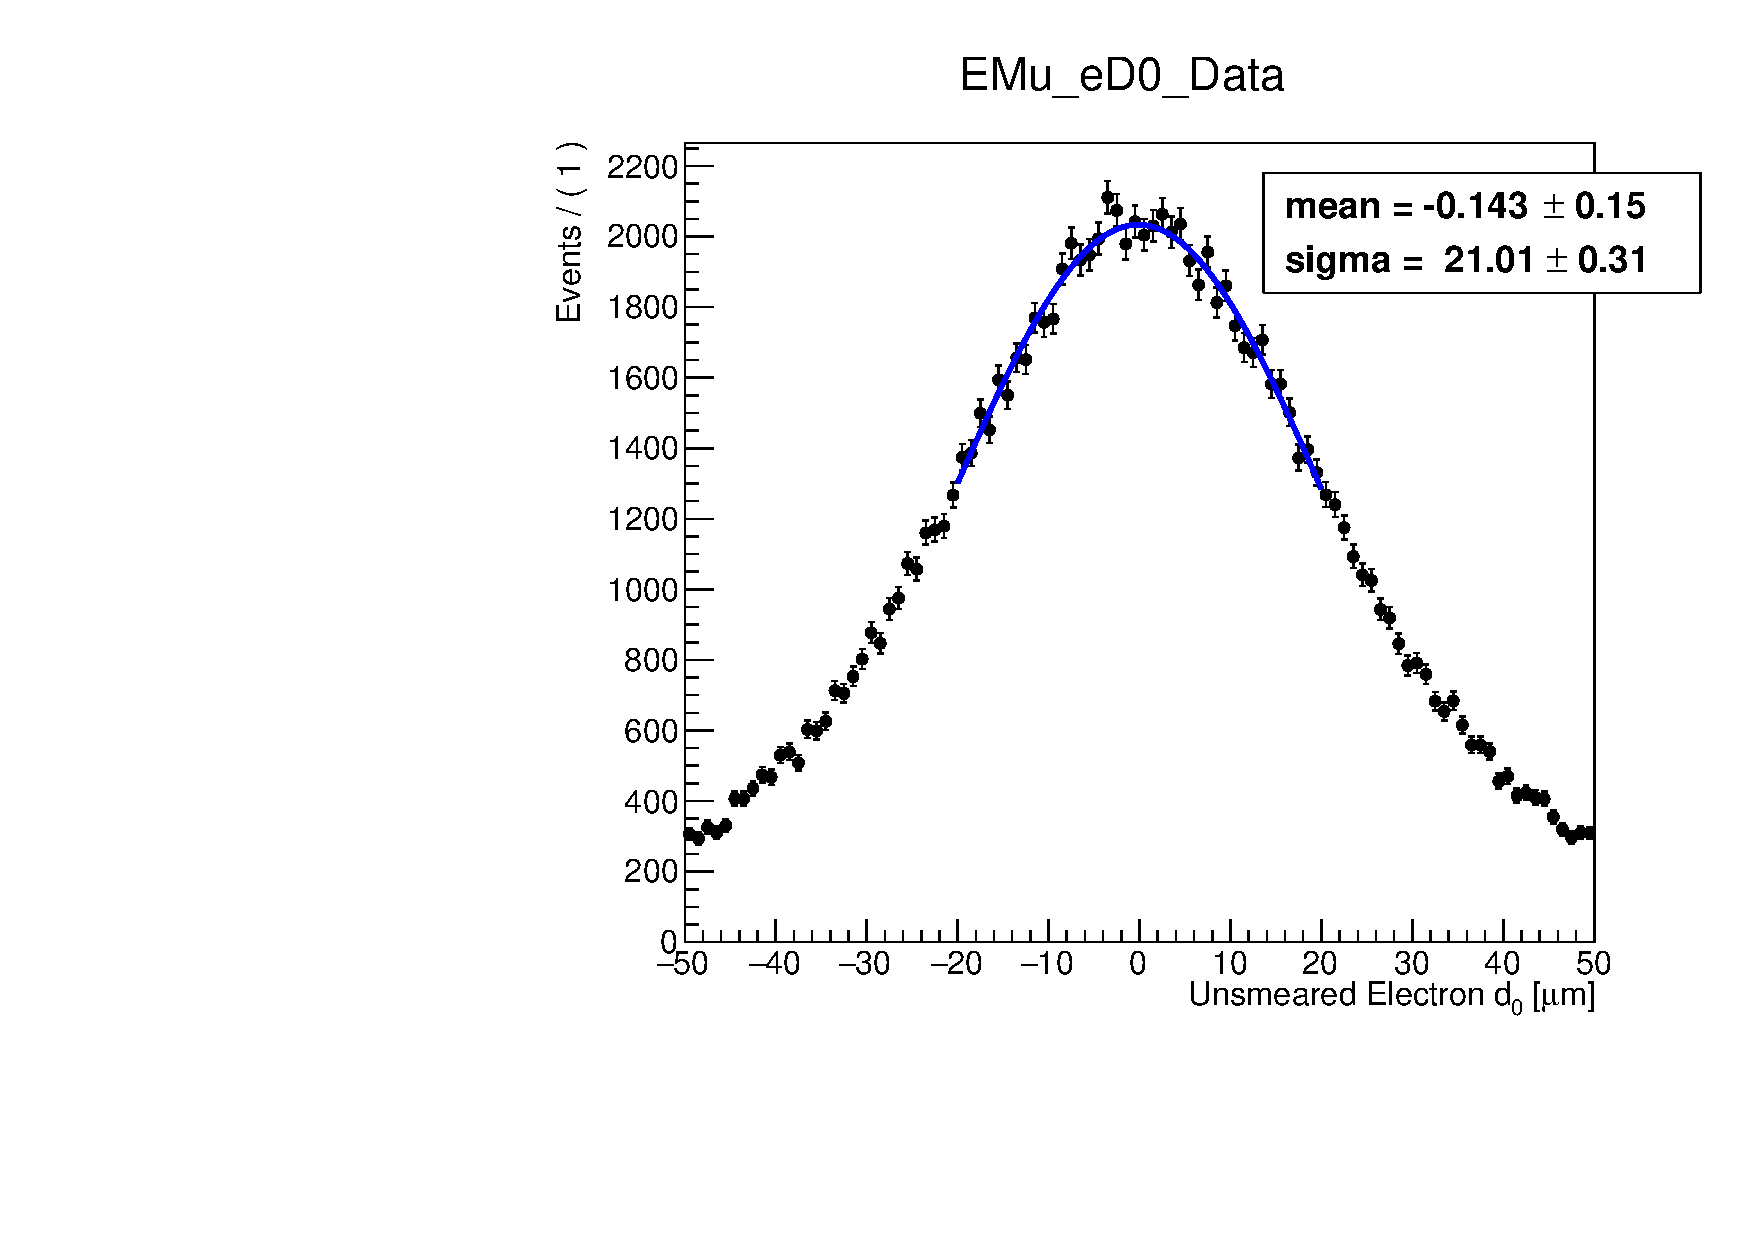
\includegraphics[scale=0.3]{figures/corrections/d0_smearing/emu_2018/gaussian_fit_EMu_eD0_Data.pdf}
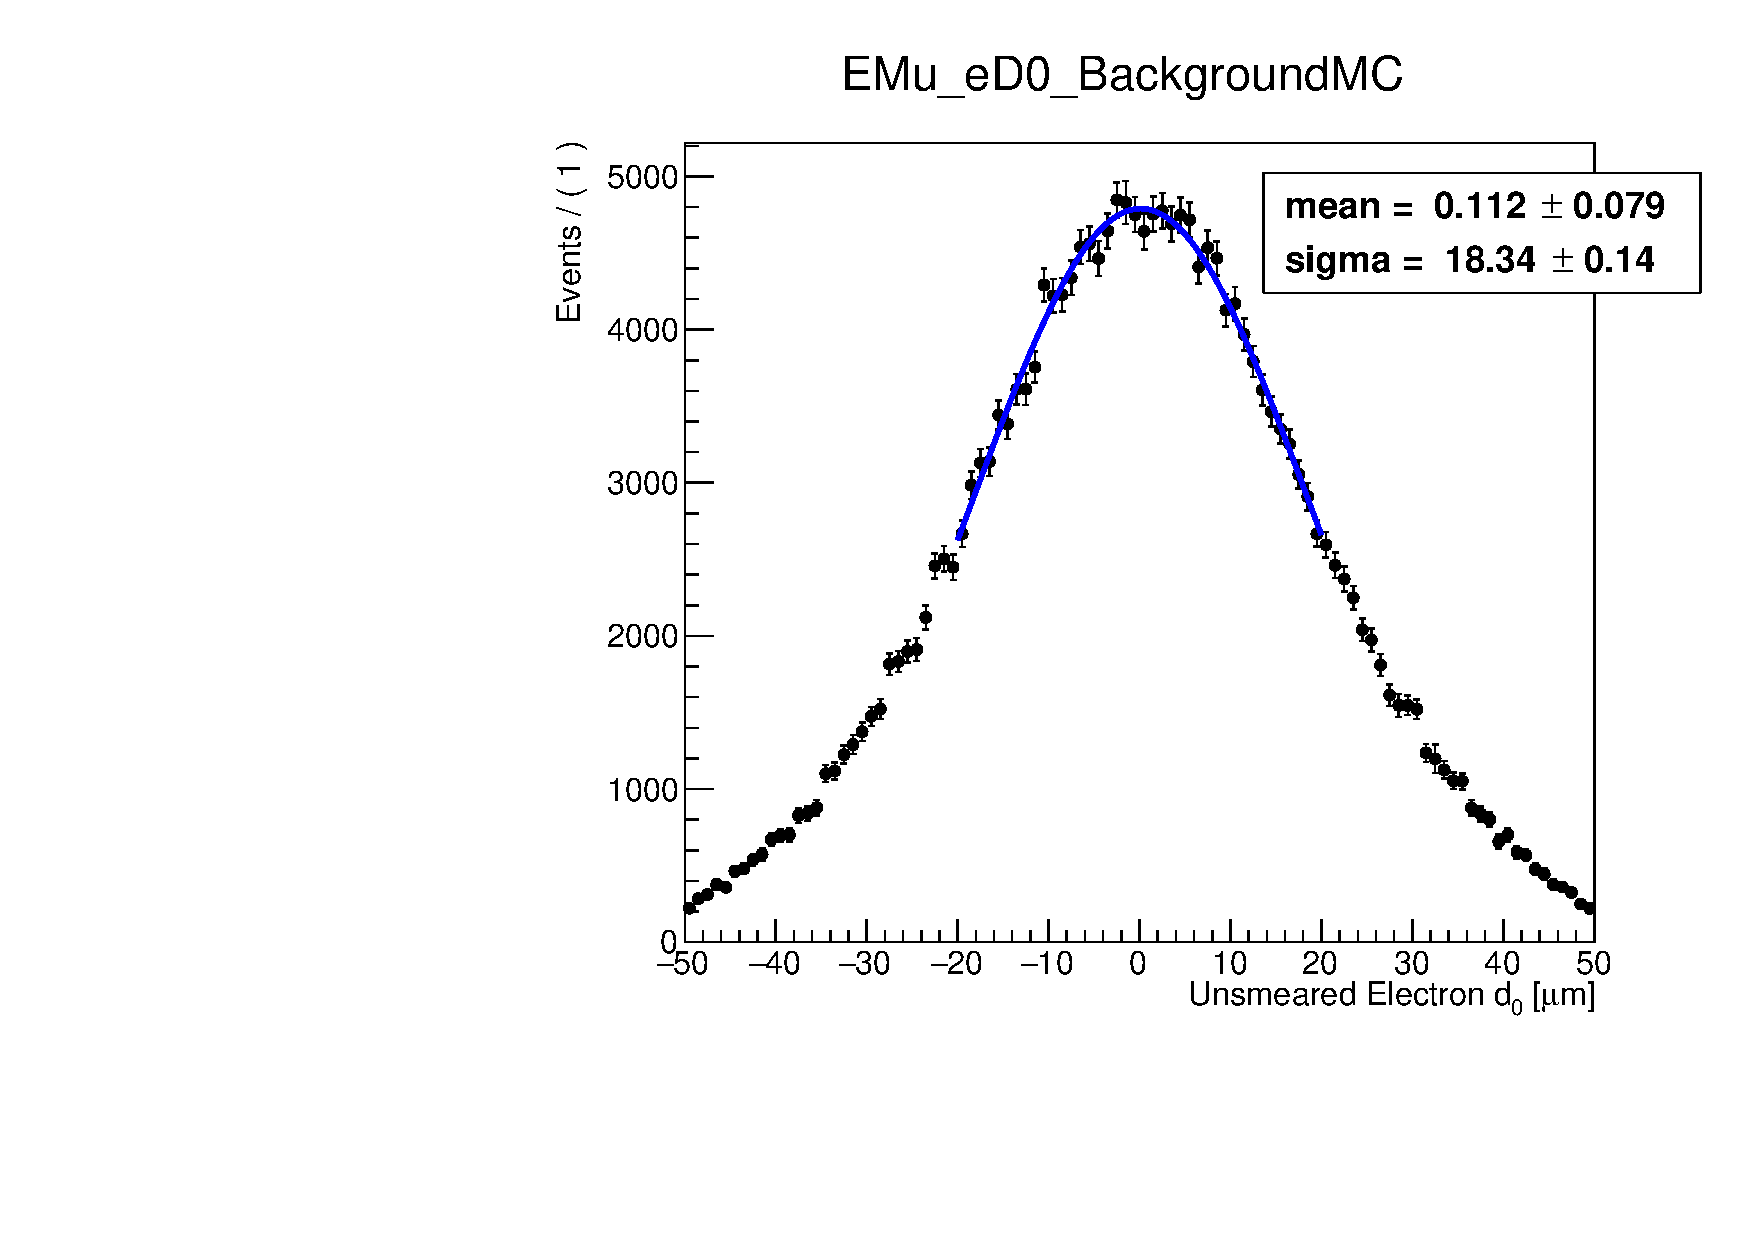
\includegraphics[scale=0.3]{figures/corrections/d0_smearing/emu_2018/gaussian_fit_EMu_eD0_BackgroundMC.pdf}
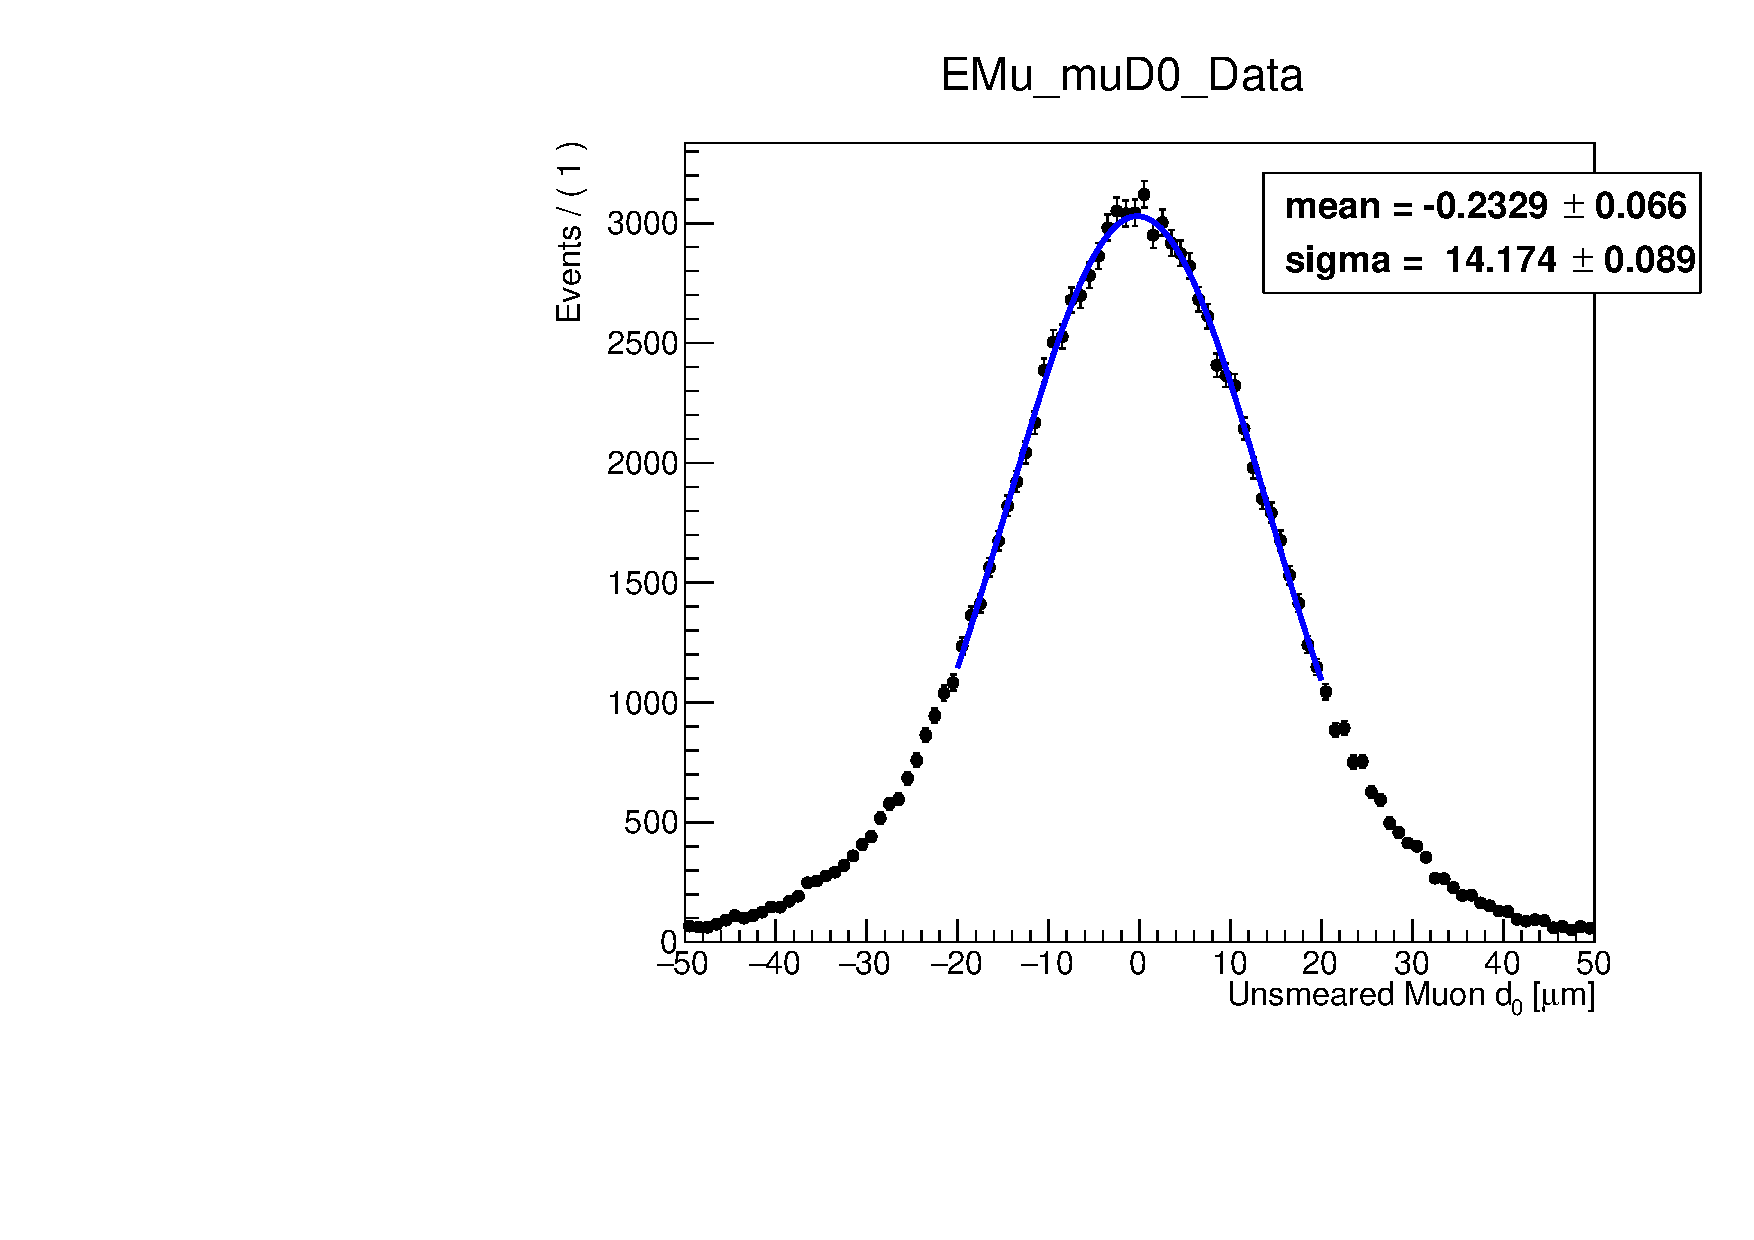
\includegraphics[scale=0.3]{figures/corrections/d0_smearing/emu_2018/gaussian_fit_EMu_muD0_Data.pdf} 
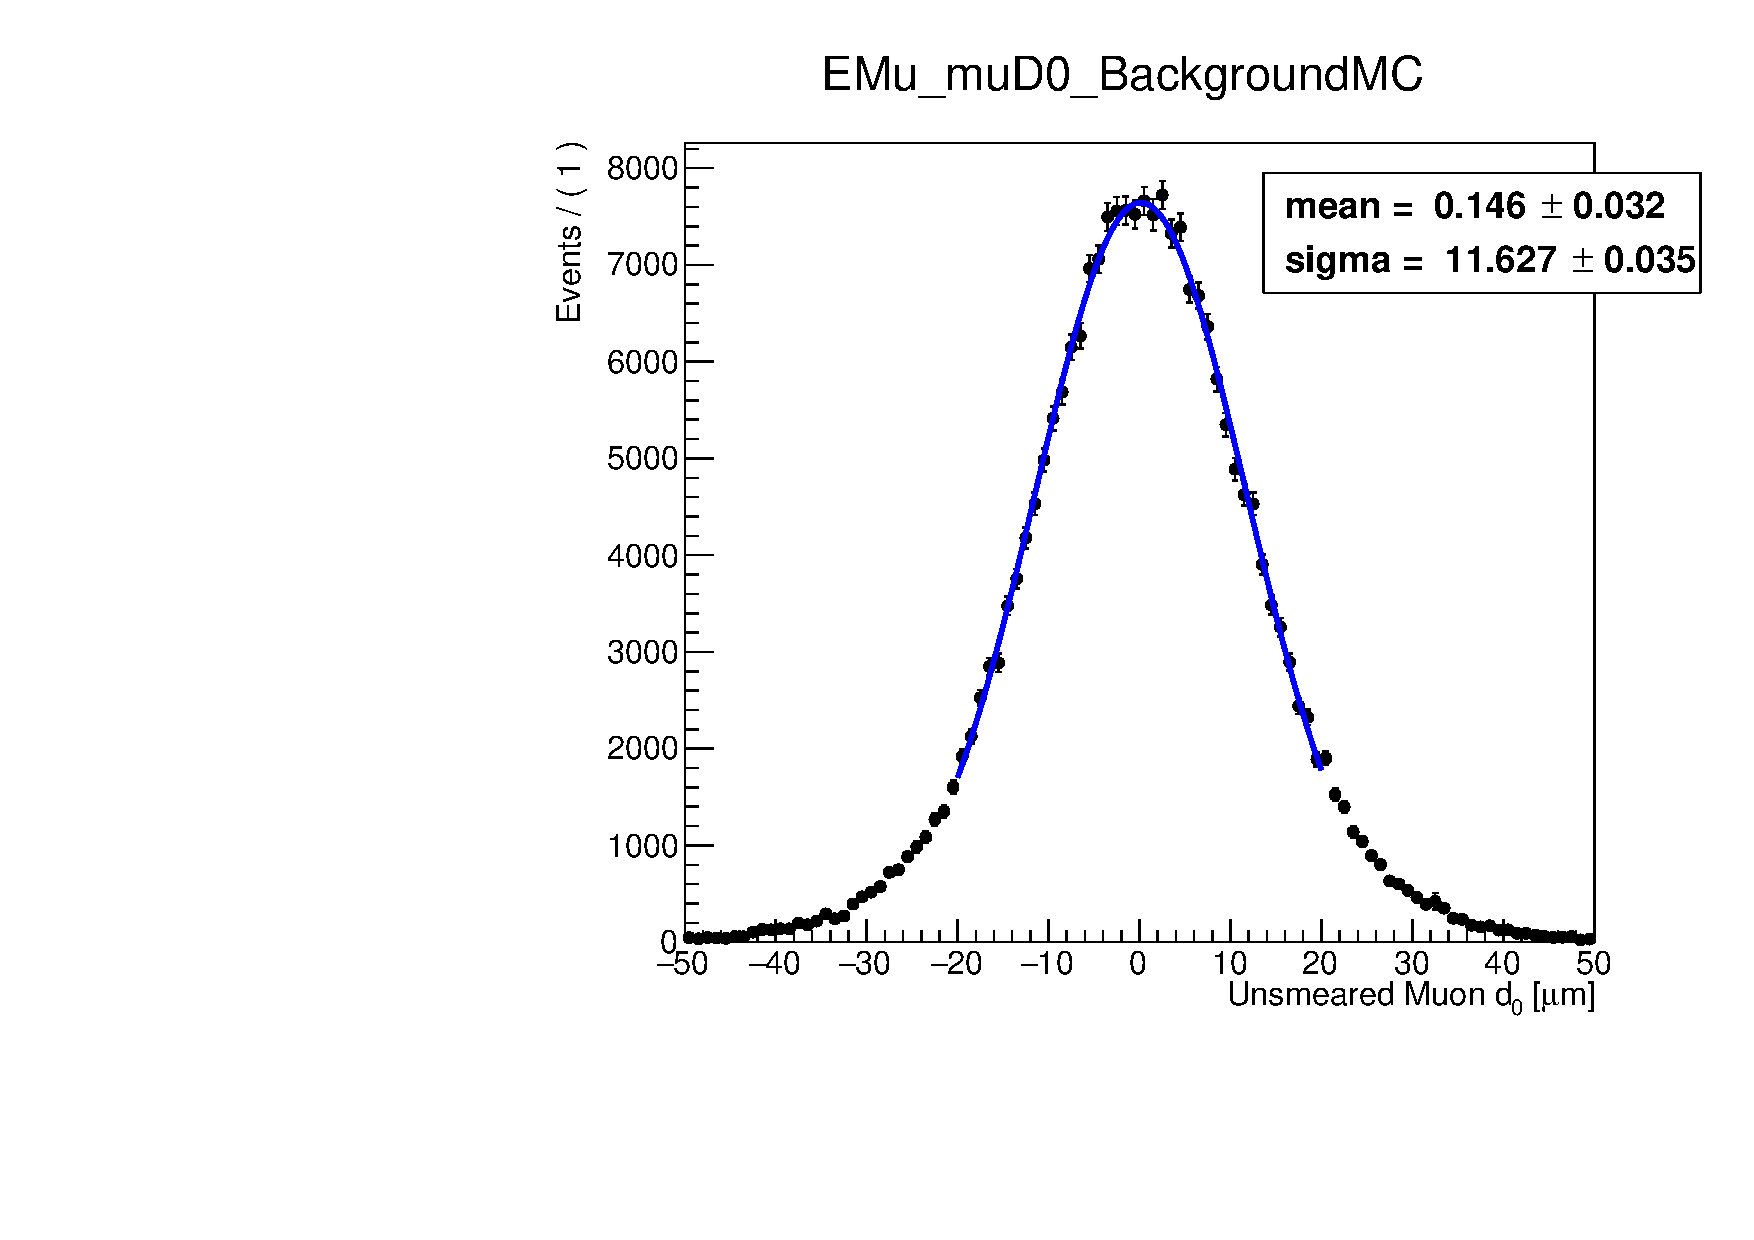
\includegraphics[scale=0.3]{figures/corrections/d0_smearing/emu_2018/gaussian_fit_EMu_muD0_BackgroundMC.pdf}
\caption{The lepton $d_0$ distributions with Gaussian fits in data (left) and background (right) for electrons (upper) and muons (lower) in the 2018 $\Pe\Pgm$ prompt control region. The widths of the Gaussian fits are used to determine the width of the Gaussian distribution used to smear the $d_0$.}
\label{gaussian_fits_2018}
\end{figure}